\section{Evaluation} \label{sec:evaluation}

In this section, we will show the results we got from our experiments. Our experiments will try to 
answer the following questions:
\begin{itemize}
    \item How is the overall throughput differ under different topologies?
    \item How is the fairness differ under different topologies?
    \item What is the conclusion of the experiment results?
\end{itemize}

The whole section is organized as the follows:
\begin{itemize}
    \item Part 1, a brief introduction of our experiment environments.
    \item Part 2, experiment results and analysis.
    \item Part 3, our suggestions according to the results we have.
\end{itemize}

\subsection{Environment Setup} \label{subsec:environment}
In our experiments, we use Mininet virtual box provided by official website\cite{Mininet:official}. 
The virtual machine runs Ubuntu Linux Quantal Quetzal on one CPU and $1024$ MB main memory.
The host machine we use has Intel\textregistered Core\texttrademark i7-3770 CPU with $12$ GB main memory running on
64-bit Windows Server 2008 R2 Enterprise version.

The network delay is set as 10{\it ms} since we simulate the network in a company, 
which typically might be higher in real-world networks \cite{NetworkDelay:web}. 
The network packet loss rate is 2\%, which is an acceptable rate as mentioned in \cite{PacketLoss:wiki}.
And all network links have a bandwidth of 100Mbps. 

We simulate each server for 10 iterations, obtaining the average results for 
analysis. Each iteration lasts for 2 minutes.

\subsection{Results and Analysis} \label{subsec:result}
We performed our experiments as discussed above. And we collected data reported by Mininet.
The notation h{\it x} where {\it x} $\in [0, 6]$ used here are the same with the ones 
shown in Figure~\ref{fig:topo}. In each table, the first column is the name of the server.
And for each client, we collected the speed value. The value is an average value of ten
experiments. And the total value in the last column means the total speed of all clients, 
which is also the overall throughput of the server. Since we have only one server in all the 
topologies, this value could be used to evaluate the overall throughput of the whole network. 
Notice that when a node is working as a server, it is not a client, that is why we have bar 
notations in the tables.

Table~\ref{table:line} here shows the result of the {\it Line Topology}. As we have 
mentioned before, there are 4 places that we can place our server in total. Let us first 
focus on only one two in the table, which means we just consider when the server is in a fixed
place, and we have some very interesting observation on different clients. Intuitively, 
the longer the distance between the server and the client, the worse the performance is. 
This is true. As we can see in the table, for the same server, as the distance grows, 
the speed of corresponding client is dropping down. However, it is not a strict linear 
relationship. For example, when {\it h0} is the server, the nearest client 
and the farthest client have distance $3$ and $8$ respectively. But the nearest client is 
almost $7.5$ times faster. Thus, when a client is closer to the server it gains far more benefit
than we expected. This is because the link between the server and the nearest client
{\it h1} is shared by all clients. Thus this link is the one with highest probability that 
congestion could happen. However, {\it h1}, the nearest client here, could take the most advantage of
this link because of the distance. Thus the speed is not a linear relationship with the distance.
This is an useful conclusion, we will use this to guide us to choose topologies later.
Figure~\ref{fig:perf-dist} shows the relationship between the throughput and the distance to
the server ({\it h0}) where the distance is represented by the distance between the switches, 
which is equal to the actual distance between hosts minus 2.

\begin{figure}[ht]
\centering 
	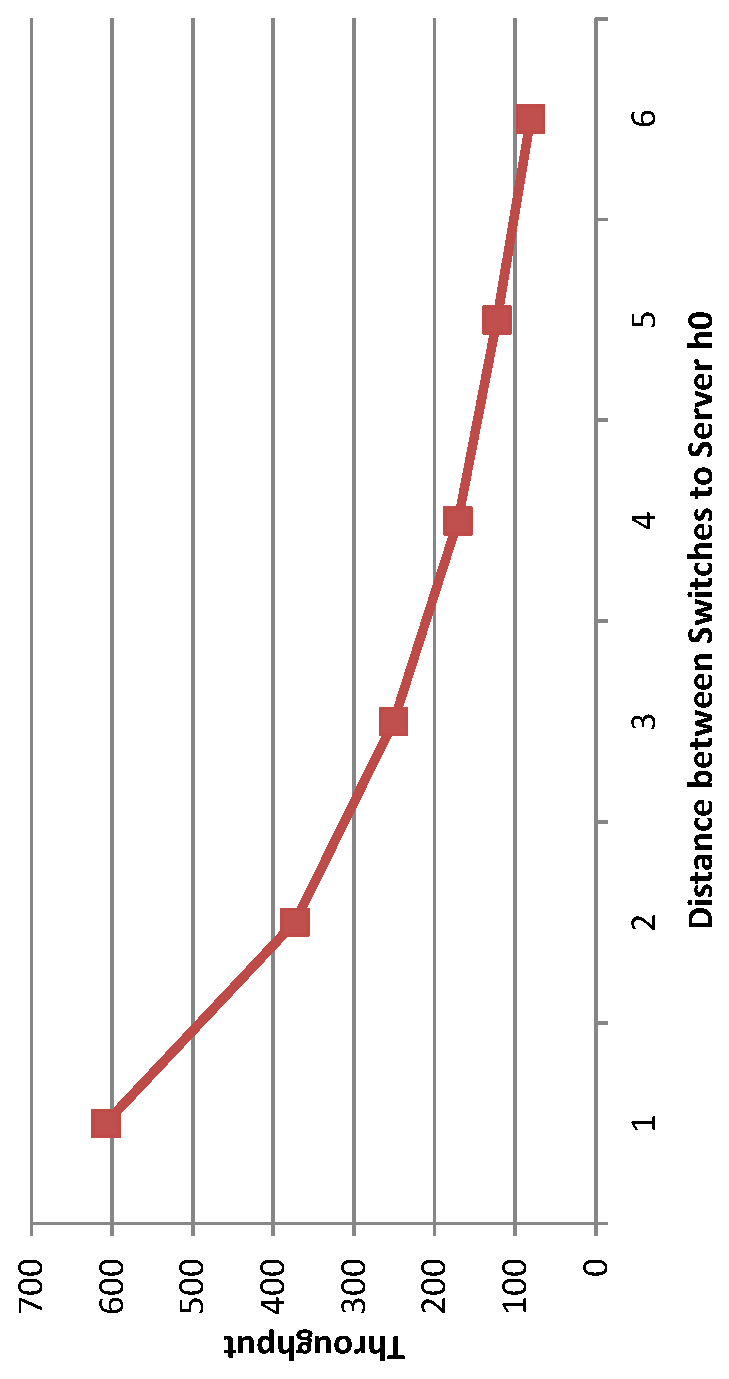
\includegraphics[angle=-90, width=0.45\textwidth, clip]{figs/performance-distance.eps}
	\caption{Relationship between Throughput and Distance for Server {\it h0} in Line Topology}
	\label{fig:perf-dist}
\end{figure}

Now let us consider different rows. It is clear that as the server moving to the center of 
the line, the overall throughput keeps growing. This is because the average distance between
server and clients becomes smaller as the server moving to the center of the line. But as we 
can see, the increasing speed is slowing down until the server reaches the center, where it 
stops growing any more.

\begin{table}
	\renewcommand{\arraystretch}{1.3}
	\caption{Line Topology}
	\label{table:line}
	\setlength\tabcolsep{4pt} % adjust the inter-column space
	\centering
	\begin{tabular}{|c||c|c|c|c|c|c|c||c|}
		\hline
		       & \multicolumn{7}{c||}{Client} &  \\ \hhline{|~||-------||~|}
		Server & h0 & h1 & h2 & h3 & h4 & h5 & h6 & Total\\
\hline\hline
h0 &     -    &  607.70  &  373.10  &  250.70  &  170.90  &  122.66  &  81.10  & 1606.16 \\
\hline
h1 &  607.50  &     -    &  610.70  &  371.20  &  245.10  &  165.22  &  113.98  & 2113.70 \\
\hline
h2 &  373.89  &  606.80  &     -    &  610.90  &  365.80  &  239.60  &  160.10  & 2357.09 \\
\hline
h3 &  243.00  &  376.40  &  611.20  &     -    &  606.70  &  371.20  &  246.20  & 2454.70 \\
\hline
	\end{tabular}
\end{table}

Table~\ref{table:star} shows the result of the {\it Star Topology}. This is a pretty
simple topology for it has only two kinds of nodes. When the center node servers as the server 
all the other nodes have almost the same speed as we can see in the table. And we also find that 
almost all client nodes have used all the bandwidth it has to communicate width the server.
Thus this is a pretty good topology if we would like to maximize our overall throughput.

However, when the server is placed at one edge. The overall throughput is not very good. This is just as
we expected. Since it has a longer distance between other edge nodes and the server. Even though 
the edge node still achieves a very good performance, the overall throughput is almost 2/3 of the
center server mode.

\begin{table}
	\renewcommand{\arraystretch}{1.3}
	\caption{Star Topology}
	\label{table:star}
	\setlength\tabcolsep{4pt}
	\centering
	\begin{tabular}{|c||c|c|c|c|c|c|c||c|}
		\hline
		       & \multicolumn{7}{c||}{Client} &  \\ \hhline{|~||-------||~|}
		Server & h0 & h1 & h2 & h3 & h4 & h5 & h6 & Total\\
\hline\hline
h0 &     -    &  612.60  &  595.70  &  608.30  &  606.50  &  611.60  &  610.60  & 3645.30 \\
\hline
h1 &  603.50  &    -     &  369.60  &  368.30  &  368.60  &  369.60  &  366.80  & 2446.40 \\
\hline
	\end{tabular}
\end{table}

Table~\ref{table:tree} here shows the result of the the {\it Tree Topology}. There are 3
different places for us to compare. For each place, the results also meet our expectations.
The distance between the server and the client is the main reason why the speed is different.
What make this topology interesting is that the overall throughput is better when {\it h1} is the 
server node instead of {\it h0}. We originally expected that {\it h0} will serve the best, because the 
average distance is smallest when {\it h0} is the server (see Table~\ref{table:distance}). 
But this is not true. We further analyzed
the result, and found that this is due to the cause we have discussed when we were analyzing
the {\it Line Topology}. The relationship between the distance and the speed is not a linear
relationship.

Let us go into details about this. Let us assume that all links has the same weight, $1$. Then,
we have $3$ types of nodes: $GN$, whose distance (hops between switches here) is $1$ and get good service from server; $MN$,
whose distance is $2$ and get medium service from server, and $BN$, whose distance is $3$ and get
bad service from the server. When {\it h0} is the server node, we have two $GN$ and four $MN$. When {\it h1}
is the server node, we have three $GN$, one $MN$ and two $BN$. Since the performance-distance 
relationship follows a concave shaped curve (see Figure~\ref{fig:perf-dist}), 
the overall throughput is dominated by $GN$ and then one $GN$ and two $BN$ are 
better than three $MN$ here. This example shows that we need to consider the distance carefully.

\begin{table}
	\renewcommand{\arraystretch}{1.3}
	\caption{Tree Topology}
	\label{table:tree}
	\setlength\tabcolsep{4pt}
	\centering
	\begin{tabular}{|c||c|c|c|c|c|c|c||c|}
		\hline
		       & \multicolumn{7}{c||}{Client} &  \\ \hhline{|~||-------||~|}
		Server & h0 & h1 & h2 & h3 & h4 & h5 & h6 & Total\\
\hline\hline
h0 &    -     &  604.10  &  600.00  &  364.30  &  372.44  &  355.30  &  369.10  & 2665.24 \\
\hline
h1 &  609.80  &     -    &  371.20  &  607.30  &  625.10  &  250.22  &  255.40  & 2719.02 \\
\hline
h3 &  372.90  &  606.30  &  240.00  &     -    &  368.90  &  170.11  &  165.33  & 1923.54 \\
\hline
	\end{tabular}
\end{table}

Now, let us compare the results among different topologies to verify the assumptions 
we made in Section~\ref{sec:approach}.

\begin{table}[ht]
\centering
	\caption{Throughput Rank to Selected Servers}
	\label{table:throughput}
	\begin{tabular}{|l||c|c|c|}
		\hline 
		Server   &  Throughput & Local Rank & Global Rank \\ \hline\hline
		Line-h0  &   1606.16  &  4   &  9 \\ \hline 
		Line-h1  &   2113.70  &  3   &  7 \\ \hline 
		Line-h2  &   2357.09  &  2   &  6 \\ \hline 
		Line-h3  &   2454.70  &  1   &  4 \\ \hline\hline 
		Star-h0  &   3645.30  &  1   &  1 \\ \hline 
        Star-h1  &   2446.40  &  2   &  5 \\ \hline\hline 
		Tree-h0  &   2665.24  &  2   &  3 \\ \hline 
		Tree-h1  &   2719.02  &  1   &  2 \\ \hline 
		Tree-h3  &   1923.54  &  3   &  8 \\ \hline 
	\end{tabular}
\end{table}
As we can see, most of the results meet our expectation. For example, {\it h0} in 
star topology is the best location to place the server and {\it h0} in line topology 
is the worst location. This proves that the average link 
distance is an important factor to consider. But we also observe some data that does not 
meet our expectation. And the reason is just like what we mentioned above: the relationship 
between the throughput and the distance is non-linear. Those results will help
us design or choose the topology we use.

\subsection{Suggestions} \label{subsec:suggestions}
According to the result we have, we have something guidance when we are facing the problem of
choosing or designing a network topology. Theoretically, the most important factor for overall 
througput to consider is the average distance between the server and all clients. The samller 
the value is, the better the overall througput is. For fairness, suppose we have the same 
average distance, we need to consider the standard deviation. It means that all clients will 
get fair services if standard deviation is samll, which means the clients has similar distances 
to the server. But we also need to consider what we have mentioned non-linear property of the two
factors. For similar average distance, the larger one may have a better overall througput. This is 
someting we have to test in real world.

Talking about real world situations, we actaully have some more things to consider. First thing and
the most important thing to consider is what is expected. For example, if all users are treated 
equally in the topology, then {\it Star Topology} with server in the center is perhaps the only 
choice. If there are some priviledged node in the topology, then we could choose others. Basically, 
we need to identify the number of different types of nodes in the topology and then follow the distribution, 
we could find the topology we want.

Other than the that, we still have some other factors to consider in real world situations. The most 
important one is that the geographically distributed buildings may limit our design or choice. And when 
we face this situations, we usually need to consider the priviledges of different departments in different 
buildings, and their priorities. This will make the problem complicated. And when we add some more factors 
like different link capabilities, we will have more complicated models.

Considering all factors, we think identifying important constrains is the most important thing to do in solving 
real world problems. When we have different constrains, different factors need to be considered. For example, 
average distance for overall throughput, standard deviation for fairness. Then, we may have some condidates. 
A simulation on a virtual network is necessary if we want to find the best solution.
